\chapter{Representative State Transfer (REST)}
\label{chap:rest}

\section{REST architecture}
\label{sec:rest-architecture}

The REST is "a set of constraints on the overall architectural approach" \cite{agile-architecture}. The goal of REST is to create a distributed hypermedia application. It is \gls{resource-based-model}, it handles with resources, the resources are named by nouns and actions are provided by HTTP requests. 

REST architecture is client-server. The server holds the implementation of logic of services and encapsulates it under the interfaces. The interfaces are entry points for client and through them he can obtain or modify the data.
REST has its best practices and constraints. The servicies built according to this definition can be called \emph{RESTful}. There are 6 constraints characterizing the REST which will be decribed further in this chapter \ref{sec:constraints}.

REST arcitecture is a composition of elements, connectors and components. None of them defines a technology but they are abstractions. The elements abstract a bahviour of components. The components have its roles, the way of interaction among them and interpretation.

The \emph{data elements} are:

\begin{description}
  \item [resource] \hfill \\ 
  Resource is an abstraction of information in REST, where any information which can be named can be a resource. "A resource is a conceptual mapping to a set of entities.." \cite{fielding} or set of values. The values can be a resource identifier and a representation.
  Resource can be static, for expamle \emph{an image}, or dynamic, \emph{the time} which dynamicaly changes and selected name for a resource is a noun (not verb).
  
  examples of resources: customer, account, ..

  \item [resource identifier] \hfill \\
  It serves to identify resources which interact with componets. The resource identifier is assigning the name thanks to which it is possible to reference appropriate resource. The identifiers is \gls{uri}, it marks a path where the resource is situated. A request form client is routed to the specific address and method which will be performed. When 
  The resource identifier for \emph{the time} then looks like: \hfill \\
There should be possible to perform the CRUD operations with the resources, every operation can be mapped on HTTP method to have its own identifier

examples:

GET     /customers      Retrives all customers
GET     /customers/5    Retrives customer with id 5
POST    /accounts       Creates new account
PUT     /accounts/13    Updates account with id 13
DELETE  /customer/2     Deletes customer with id 2   

 
  resource identifiers 
  \texttt{http://www.api.com/time}
  \item [representation] \hfill \\
  Rapresentation is used by REST components to perform changes to the resource. Format of representations data is called media type and have influence on the performance of the hypermedia. Media types can be proprietary or standardized, from standardized types there are for comparison \gls{xml} and \gls{json}. JSON format is less verbose then XML and in consequence in sake of data transmission it would be performed faster than a XML representation fomat.
  Example of representation:
  \begin{description}
    \item[In plain text] \texttt{Mon Nov 29 2014 18:03:19 GMT+0100}
    \item[In xml format] \texttt{<time>2014-11-29T18:03:19+01:00</time>}
  \end{description}
  \item [representation metadata] \hfill \\
  This metadata describes the data of which the represenation consists of.
  Examples: \hfill \\
  \texttt{Content-Type: text/plain} \hfill \\
  \texttt{Content-Type: text/xml}
   \item [resource metadata] \hfill \\
  Resource metadata stores an information about the resource that is not specific to the supplied representation.
  Example: \texttt{Allow: GET}
  \item [control data] \hfill \\
  Control data decribes the purpose of a message between components, for expamle \emph{GET} and parametizes the request, for expample to define casheability. 
\end{description}

The \emph{connectors} provides the access point for the values of the resource. In connectors belong client, server, cache, resolver, tunnel. %TODO explanation, mabye image

REST \emph{components} are an abstraction of application unit. The components are origin server, gateway, proxy, user agent. %TODO explanation, mabye image

\bigskip

Every resource has its representation, it describes how resources get manipulated in RESTful API architecture. The representation represents part of (or less commonly the whole) resource state, it is transferred between the client and server and has generally the JSON or XML format, but could be in many other formats as well. The representation is composed from resource and attached files which provide enough information for the client to be able to modify the resource on the server.

\section{REST constraints}
\label{sec:constraints}

Six constraints that are applied to the architecture to create RESTful services. Respecting this rules leads to desiderable properties of the system, such as performance, scalability, simplicity, modifiability, visibility, portability and reliability. 
%%(citacia http://www.restapitutorial.com/lessons/whatisrest.html#)
\begin{description}
  \item The six constraints are:
  
%TODO write about HATEOAS

\begin{enumerate}
  \item Uniform Interface
  
Define interface between client and server. It separates client and server allowing them to develop each part independently. The interface is uniform, so that is easy to understand for both, the server and the client.
Interface is resource-based - requests in \gls{uri} contain the resource identifiers which identifies the concrete resource. To the client is then sent the representation which is conceptually separated from the resource. The representation is commonly XML or JSON format and represents appropriate database record.
Resources are manipulated exclusively throught the rapresentations. The representation with any metadata attached, keeps enough information for the client and allow him to modify the resource on the server.
The sentmessage which represents the request sent by client or the response form the server is self-decriptive. That means there is enough information to know hov to process the message and the response explicitely defines the cashability.
The representation is sent using \emph{\gls{http} specification}, client call the resource using HTTP verbs (GET, POST, PUT, DELETE,..) and the URI, server sends to the client the HTTP response.
The REST is not restricted only on the four HTTP methods, a service can implement its own methods, for example \texttt{GetByName}. The repsponse would be representation of resource corresponding to the name parameter contained in the request.

  \item Stateless
  
Each message is self-descriptive, a request has enough context to be understand so that the messages has no state. Any state of a \gls{session} is held just on the client side.
The statelessness allows greater scalability, because server doesn't have to cammunicate with the session, which can be created to carry the state using another architectural style of services. Relaibility is improved because of easier recovery of partial failures. Disadvantage is that the requsts which are sent contain repetitive data and the server has lower control over the application behaviour.

\item Client-server

RESTful architecture is client-server architecture. There are two disconnected concerns, it is properly defined what is user interface and services. Client can’t have direct access to the database, assets or resources, which improves the portability of client code. Servers are not included in uder interface, which improves the simplicity and scalability of server-side code. Uniform interface links the client and server together. The two concerns can be developed indipendently as long as the interface is not altered. 

\item Casheable

Server responses (representations) are casheable, everything that comes back to server or from REST service could be casheable. Responses are able to to define themselfs as cashable implicitly (it’s not noted in general client), explicitly (server specifies) or negotiated (to figure out how long can be cashed), to avoid the inappropriate reuse of data contained in response in further requests. Cashing partially limits the clinet-server interaction but improves the scalability and performance. 
Picture \ref{fig:casheability} describes possible options of casheability.

%TODO rewrite 

\begin{figure}[htp] \centering{
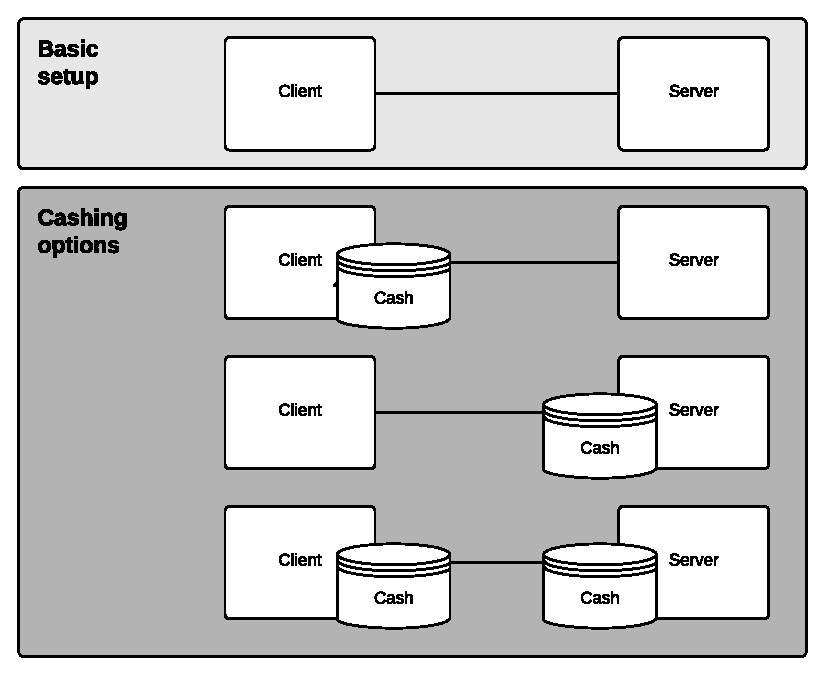
\includegraphics[width=12cm]{img/casheability.pdf}}
\caption{Casheability options}
\label{fig:casheability}
\end{figure} 

\item Layered system

Linked to cashability and client-server constraints. Client is not able to see if he is communicating diractly with the server, or with an intermedia between them. Intermedia improves scalability, provide shared cashes and morover can enforce the security policies.

\item Code on demand (optional)

The logic can be transferred to the client-side, this way the server can temporarily extends or customize the functionality of the client. This can be performed for example by the components like service-side scripts.
This constraint is unique, it is the only one which can be violated and the services can be still reffered as RESTful.

\end{enumerate}
\end{description}

\bigskip
\section{Application of REST}

Having the SOA and knowing the constraints of the REST services can be designed. When a company wants to develop a system with RESTful services it has to apply at least the first five of constraints. But it can occure that not all the constraints are profitable for an application. In this case the architecture can forget some of them but the services cannot be further marked as RESTful. This notation doesn't affect services themselfs, the result can be still the best design for current application.

\subsection{RESTful service example}
There is a cropration with SOA and its services are designed according to REST constraints. One of the services is representing bussiness abstraction of \emph{customers} of the company. Customers can be viewed, created, modified or deleted. For this goal the HTTP requests are used (GET, POST, PUT, DELETE). 

In designing the service there will be considered the notation of \gls{webapi} \gls{framework}. 

Resource identifier is a URI address. In ASP.NET Web API is composed from \emph{controller}, which is a class handling the HTTP request and a method of the controller which is called \emph{action}. In case of customer service example the controller is \emph{customer}, the action can be \emph{GET} and to identify a specific customer the parameter \emph{name} as to be a part of URI.

\lstset{frame=none,
  language=JAVA,
  aboveskip=3mm,
  belowskip=3mm,
  showstringspaces=false,
  columns=flexible,
  basicstyle={\small\ttfamily},
  numbers=none,
  breaklines=false,
  breakatwhitespace=false,
  tabsize=3
}

\begin{lstlisting}
GET customers/getByName/{name} 
\end{lstlisting}

When the client wants to get the customer whose name is \emph{Peter} then the request looks like:

\begin{lstlisting}
GET customers/getByName/Peter 
\end{lstlisting}

Thanks to URI the request is roated to specific resource and returns a response. This response is a representation containing customer with the requested name. Represenation has its media type which are stated in the metadata in this case it is for example JSON format:

\begin{lstlisting}
{ id: 2,
name: "Peter",
surrname: "Sun",
e-mail: "peter.sun@service.com" }
\end{lstlisting}

%!TODO 
%%\footnote{Technologie jsou popsány v sekci~\ref{sec:technologies}.} 


